\documentclass[10pt,conference,compsocconf]{IEEEtran}

\usepackage{hyperref}
\usepackage{graphicx}	% For figure environment
\usepackage{amsmath}
\usepackage{amssymb}

\begin{document}
\title{Higgs Boson Detection}

\author{
  Beuchat Bastien, Mamie Robin, Mion Jeremy\\
  \textit{CS-433: Machine Learning (Fall 2019),}\\
   \textit{École Polytechnique Fédérale de Lausanne, Switzerland}
}

\maketitle

\begin{abstract}
In the first project of the EPFL Machine Learning course, six different algorithms were implemented to solve the provided challenge: predict from CERN experimental data whether a particle is a Higgs boson or not.

For this purpose, the required functions were implemented, evaluated, and fine-tuned using cross-validation.
The provided data had to be processed using diverse feature expansion techniques and partitioning.
\end{abstract}


\section{Introduction}

The aim of this project is to create a binary classifier that will separate Higgs boson's detection from simple background noise.
A data-set containing 250'000 observations from CERN, with each 30 different features, was provided to train the machine learning algorithms.


\section{Methodology}

The data had to be firstly explored and understood.
Since none of the writers of this report are physicists, the exact meaning of each column in our data-set was not completely understood from the beginning.
The prevalence of the features, or whether there is some link between them, was the goal of this first exploration.

Once we acquainted ourselves with the provided data-set, the data processing began.
First, the essential preparation was done: normalisation and handling of the unavailable values.
Then, the machine learning algorithms were implemented.
Once ready, they were trained and evaluated to see whether their implementation was at least correct.
After this, we prepared our data differently in order to get more accurate models with more carefully prepared data-sets.
To train sufficiently good models, we had to define their hyper parameters.
For this task, cross-validation was done across all algorithms.


\section{Data Preparation}

\subsection{Data Parsing}

The first step of data preparation was handling unavailable data.
Indeed, in the data-set, there were unavailable data for some features of some observations.
The observations and features at fault could not simply be dropped, because non-existing data is an information that had to be taken into account.
The first applied strategy was to replace unavailable data by the mean of their respective feature.

A more meaningful technique was then found.
In the data-set documentation \cite{higscern}, it is specified that unavailable data depends on PRI\_jet\_num  values and that the data-set can be broken into 4 different parts.
Most of the variables of these new data-sets are defined; some variables are occasionally null because CERN could not calculate them.

They were then normalised.
This has the great effect of reducing the magnitude of the values and improving the stability of the computations, i.e. the values overflow less quickly when the data is given to the machine learning algorithms. At this point, the data was ready for a first evaluation.

Measuring the accuracy of our initial model (see table \ref{acc table}) allowed us to see that ridge regression was the most promising algorithm. The improvements will be focused on improving the ridge regression algorithm.


\section{Improvements}


\subsection{Special Case: the Mass} \label{mass}

A significant amount of DER\_mass\_MMC measurements are not defined.
CERN \cite{higscern} indicates that this is the case when "the topology of the event is too far from the expected topology".
From this information, the goal is to find out whether whether the mass is a useful variable to distinguish Higgs bosons from background noise.

\begin{figure}[h]
    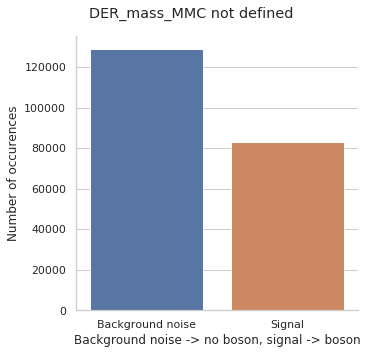
\includegraphics[width=4cm]{DER_mass_MMC_defined.png}
    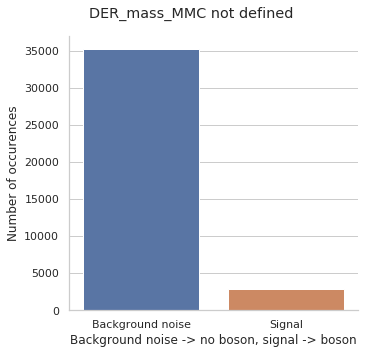
\includegraphics[width=4cm]{DER_mass_MMC_not_defined.png}
    \caption{Ratio difference between signals and background noise when DER\_mass\_MMS is defined or not.}
    \centering
    \label{mass_occurence}
\end{figure}

It can be clearly seen from Figure \ref{mass_occurence} that the absence of any mass measurement is a very useful feature to detect background noise.


\subsubsection{Variable Expansion}\label{variable expansion}

The first feature expansion idea was adding a variable representing the fact that DER\_mass\_MMC  is defined or not.
This helped improve our accuracy to 0.7584.


\subsubsection{Splitting on DER\_mass\_MMC} \label{split mass}

Since the accuracy improvement was quite noticeable, the decision was made to split our four data-sets using the presence of DER\_mass\_MMC or lack thereof.
One half represents the presence of any DER\_mass\_MMC measurement, and the other the absence.
This yielded 8 different data-sets on which we could train our models.
This split yielded results with an accuracy of 0.7584 which is better than in part \ref{variable expansion}.

The decision was made to keep the data-set split into 8 as described in this section, discarding the work done in \ref{variable expansion} made redundant by this splitting.


\subsection{Feature Expansion}

\subsubsection{Non Linear}

Given the importance of DER\_mass\_MMC noticed in \ref{mass}, the decision was made to add a new feature to our data-set.
This new feature is defined as follows:

$$ \frac{\textrm{DER\_mass\_MMC} * \textrm{DER\_pt\_ratio\_lep\_tau}}{(\textrm{DER\_sum\_pt}+1e-10)} $$

We wanted to use 2 other DER features since according to the CERN paper \cite{higscern} these were selected by physicists at ATLAS and derived from the primitive features. We are assuming the the physicists know what they are doing and gave us useful features. Adding a small constant in the denominator allows us to ensure that we are not going to divide by zero.
This new feature allowed us to increase the accuracy of our model to 0.7653.

\subsubsection{Polynomial}

Different degrees of polynomial expansion were tested to determine what was ideal.
The polynomial expansion is defined as:

$$ f(X) = [ XX^2 \cdots X^d], \quad d \in \mathbb{N}, \, X \textrm{ is our feature matrix}  $$

To apply the polynomial expansion while keeping the computations numerically stable we chained our normalisation steps with our expansion step as follows:

$$\textrm{normalise} \xrightarrow{} \textrm{polynomial expansion} \xrightarrow{} \textrm{normalise} $$

The accuracy of our model was measured by taking 10\% of our data and setting it aside for the final evaluation of our model's accuracy. Table \ref{accuracy} shows the different degrees tested for polynomial expansion.

\begin{table}[t]
\caption{Accuracy was measured by using a 10\% validation set of ridge regression.}
\begin{tabular}{|c|c|c|c|c|l}
\hline
\textbf{Degree} \textit{d}   & 1      & 3      & 4      & 5      & \multicolumn{1}{c|}{6}      \\ \hline
\textbf{Accuracy} & 0.7646 & 0.7941 & 0.8112 & 0.8138 & \multicolumn{1}{c|}{0.8132} \\ \hline 
\textbf{Degree} \textit{d}   & 7      & 8      & 12     & 16     &                             \\ \cline{1-5}
\textbf{Accuracy} & 0.8124 & 0.8115 & 0.8099 & 0.8084 &                             \\ \cline{1-5}
\end{tabular}
\centering
\label{accuracy}
\end{table}

After testing, see table \ref{accuracy}, the decision was made to set the degree to five as it provided the most accurate model.

\subsection{Combining PRI\_jet\_num }

After further review of our dataset, it was noticed that all the features that are defined when PRI\_jet\_num = 2 are also defined when PRI\_jet\_num = 3.
We therefore decided to merge these models to see if it improved our accuracy, which it did. The accuracy with this improvement was 0.8153.

\begin{table}[ht]
\caption{Accuracy of all our algorithms.}
\begin{tabular}{|c|c|c|c|}
\hline
\textbf{Algorithm}                                                               & \textit{Least-square GD}  & \textit{Least-square SGD}                                                             \\ \hline
\textbf{\begin{tabular}[c]{@{}c@{}}Accuracy without\\ improvements\end{tabular}} & 0.6930                    & 0.6930                                                                                \\ \hline
\textbf{\begin{tabular}[c]{@{}c@{}}Accuracy with \\ improvements\end{tabular}}   & 0.7397                    & 0.7397                                                                                \\ \hline \hline
\textbf{Algorithm}                                                               & \textit{Least squares}  & \textit{Ridge regression}                                                               \\ \hline
\textbf{\begin{tabular}[c]{@{}c@{}}Accuracy without\\ improvements\end{tabular}} & 0.7573                  & 0.7576                                                                                  \\ \hline
\textbf{\begin{tabular}[c]{@{}c@{}}Accuracy with \\ improvements\end{tabular}}   & 0.8187                  & 0.8153                                                                                  \\ \hline \hline
\textbf{Algorithm}                                                                & \textit{Logistic regression} & \textit{\begin{tabular}[c]{@{}c@{}}Regularized logistic\\ regession\end{tabular}} \\ \hline
\textbf{\begin{tabular}[c]{@{}c@{}}Accuracy without\\ improvements\end{tabular}} & 0.7329                       & 0.6930                                                                             \\ \hline
\textbf{\begin{tabular}[c]{@{}c@{}}Accuracy with\\ improvements\end{tabular}}    & 0.8206                       & 0.7397                                                                             \\ \hline
\end{tabular}
\label{acc table}
\centering
\end{table}

\section{Experiments}

K-fold cross-validation was used on our models to yield the best hyper-parameters possible.

The vast majority of our algorithms fared well when given these new and improved data-sets, having their success rate greatly improved.
However, an algorithm in particular did not give any good result after the massive polynomial expansion, namely the least squares function.
Indeed, the condition number of the matrix went on the rise, coming from ca. $10^{12}$ to $10^{18}$.
This causes the algorithm to give incoherent results when using the defined data-sets.

In the logistic regression algorithms, a threshold was added in order not to give values that are too big to the sigmoid function.
Anything above 20/below -20 was simply mapped to 20/-20, since the output of the sigmoid will be very close to 1/0 in these cases.
This allowed the program to not suffer from any overflow in the exponential part of the sigmoid, and to have well-defined values in the logarithm used in the loss/gradient computation.

\section{Conclusion}

The algorithm that saw the biggest increase of accuracy with our experiments was the ridge regression.
With a peak of classification at 81.4\%, it was our best attempt at classifying the problem. According to table \ref{acc table}, logistic regression appears to be a better solution but handing it in to Aicrowd only yields an accuracy of 72.7\%.

\newpage

\begin{thebibliography}{9}
    \bibitem{higscern} 
    Learning to discover: the Higgs boson machine learning challenge
    \\
    \footnotesize{https://higgsml.lal.in2p3.fr/files/2014/04/documentation\_v1.8.pdf}
\end{thebibliography}

\end{document}